% questions.tex —— 1997 年·上海卷·理工农医类 · 题目内容片段（无答案）
% 由 tools/generate_projects.py 依来源总账自 1997/1997_数学真题_上海理_试题.md 生成，勿手改（改源 MD 后重跑）


\begin{gktip}
来源说明：本稿按固定来源 PDF 第 1–4 页转录题面，第 4–7 页为「答案要点」。扫描件无文字层，上下标、分数线与图形按 300 dpi 渲染逐题核对；来源身份为「1997 年全国普通高等学校招生统一考试·上海数学试卷（理工农医类）」，出版者/版次未核实，故答案标作「来源印载答案」。全卷 22 题：选择 1–6（每题 4 分）、填空 7–16（每空格 4 分，13–16 为 $A_1$/$B_1$ 选做）、解答 17–22（10+10+14+16+18+18 分，20 为 $A_2$/$B_2$ 选做），满分 150 分。

考生须知（节录）：全卷 22 题、满分 150 分；选做题按 $A_1$/$A_2$ 组与 $B_1$/$B_2$ 组排列，考生从对应的两组中选做一组，若同时做两组或分别做两组中的部分试题，则只对 $A$ 组中所完成的部分评分（计分）。选择题「不选、选错或者选出的代号超过一个（不论是否都写在圆括号内），一律得零分」。

图形说明：第 18、19、20 $B_2$、21 题的 TikZ 图稿依原页可辨认的拓扑、标号与关系重绘，不宣称按比例测绘。
\end{gktip}

来源题签：“1997 年全国普通高等学校招生统一考试·上海数学试卷（理工农医类）”。固定来源 PDF 共 7 页；扫描件首页标明全卷 22 题、满分 150 分。本文按来源扫描页转录，题面与来源身份均待独立核对；出版者及印载答案的官方身份尚未核实。选择题 1—6，填空题 7—16，解答题 17—22。全卷含 $A_1$/$B_1$、$A_2$/$B_2$ 两组对应选做题，按原卷说明选择。

\gkpart{一、选择题（1—6，每题 4 分，共 24 分）}

\begin{question}
\gkti{1}设全集是实数集 $\mathbb R$，$M=\{x\mid x\le 1+\sqrt2,\ x\in\mathbb R\}$，$N=\{1,2,3,4\}$，则 $\overline M\cap N$ 等于\mbox{（　　）}

（A）$\{4\}$　（B）$\{3,4\}$　（C）$\{2,3,4\}$　（D）$\{1,2,3,4\}$

\end{question}
\begin{question}
\gkti{2}三个数 $6^{0.7}$、$0.7^6$、$\log_{0.7}6$ 的大小顺序是\mbox{（　　）}

（A）$0.7^6<\log_{0.7}6<6^{0.7}$　（B）$0.7^6<6^{0.7}<\log_{0.7}6$

（C）$\log_{0.7}6<6^{0.7}<0.7^6$　（D）$\log_{0.7}6<0.7^6<6^{0.7}$

\end{question}
\begin{question}
\gkti{3}在下列命题中，假命题是\mbox{（　　）}

（A）若 $a,b$ 是异面直线，则一定存在平面 $\alpha$ 过 $a$ 且与 $b$ 平行。

（B）若 $a,b$ 是异面直线，则一定存在平面 $\alpha$ 过 $a$ 且与 $b$ 垂直。

（C）若 $a,b$ 是异面直线，则一定存在平面 $\alpha$，与 $a,b$ 所成角相等。

（D）若 $a,b$ 是异面直线，则一定存在平面 $\alpha$，与 $a,b$ 的距离相等。

\end{question}
\begin{question}
\gkti{4}设 $\theta\in\left(\dfrac{3\pi}{4},\pi\right)$，则关于 $x,y$ 的方程 $x^2\csc\theta-y^2\sec\theta=1$ 所表示的曲线是\mbox{（　　）}

（A）实轴在 $y$ 轴上的双曲线　（B）实轴在 $x$ 轴上的双曲线

（C）长轴在 $y$ 轴上的椭圆　（D）长轴在 $x$ 轴上的椭圆

\end{question}
\begin{question}
\gkti{5}如果直线 $l$ 沿 $x$ 轴负方向平移 3 个单位，再沿 $y$ 轴正方向平移 1 个单位后，又回到原来的位置，那么直线 $l$ 的斜率是\mbox{（　　）}

（A）$-\dfrac13$　（B）$-3$　（C）$\dfrac13$　（D）$3$

\end{question}
\begin{question}
\gkti{6}设 $f(n)=\dfrac1{n+1}+\dfrac1{n+2}+\dfrac1{n+3}+\cdots+\dfrac1{2n}$（$n\in\mathbb N$），那么 $f(n+1)-f(n)$ 等于\mbox{（　　）}

（A）$\dfrac1{2n+1}$　（B）$\dfrac1{2n+2}$

（C）$\dfrac1{2n+1}+\dfrac1{2n+2}$　（D）$\dfrac1{2n+1}-\dfrac1{2n+2}$

\end{question}
\gkpart{二、填空题（7—16，每题 4 分，共 40 分）}

\begin{question}
\gkti{7}二次曲线 $\begin{cases}x=5\cos\theta,\\ y=3\sin\theta\end{cases}$（$\theta$ 是参数）的左焦点坐标是 \gkblank{}。

\end{question}
\begin{question}
\gkti{8}方程 $\sin 2x=\dfrac12$ 在 $[-2\pi,2\pi]$ 内解的个数是 \gkblank{}。

\end{question}
\begin{question}
\gkti{9}已知 $a=\dfrac{-3-i}{1+2i}$（$i$ 是虚数单位），那么 $a^4=$ \gkblank{}。

\end{question}
\begin{question}
\gkti{10}设圆 $x^2+y^2-4x-5=0$ 的弦 $AB$ 的中点为 $P(3,1)$，则直线 $AB$ 的方程是 \gkblank{}。

\end{question}
\begin{question}
\gkti{11}若 $(3x+1)^n$（$n\in\mathbb N$）的展开式中各项系数的和是 256，则展开式中 $x^2$ 的系数是 \gkblank{}。

\end{question}
\begin{question}
\gkti{12}函数 $f(x)=3\sin x\cos x-4\cos^2x$ 的最大值是 \gkblank{}。

\end{question}
\gksubpart{选做题：$A_1$组与$B_1$组二选一}

原卷说明：$A_1$组适合非试点校考生，$B_1$组适合试点校考生；考生从两组中选做一组。

\begin{question}
\gkti{13}

$A_1$组（非试点校）：设 $0<a<b$，则 $\displaystyle\lim_{n\to\infty}\frac{4b^n}{a^n-b^n}=$ \gkblank{}。

$B_1$组（试点校）：$\displaystyle\lim_{n\to\infty}\left(1-\frac2n\right)^{-2n}=$ \gkblank{}。

\end{question}
\begin{question}
\gkti{14}

$A_1$组（非试点校）：设正四棱锥底面边长为 $4\,\mathrm{cm}$，侧面和底面所成的二面角是 $60^\circ$，则这个棱锥的侧面积是 \gkblank{} $\mathrm{cm}^2$。

$B_1$组（试点校）：设 $\vec a=(m+1)\vec i-3\vec j$，$\vec b=\vec i+(m-1)\vec j$，$(\vec a+\vec b)\perp(\vec a-\vec b)$，则 $m=$\gkblank{}。

\end{question}
\begin{question}
\gkti{15}

$A_1$组（非试点校）：圆柱形容器的内壁底半径为 $5\,\mathrm{cm}$，两个直径为 $5\,\mathrm{cm}$ 的玻璃小球都浸没于容器的水中。若取出这两个小球，则容器内的水面将下降 \gkblank{} $\mathrm{cm}$。

$B_1$组（试点校）：设 $f(x)=x^2(2-x)$，则 $f(x)$ 的单调递增区间是 \gkblank{}。

\end{question}
\begin{question}
\gkti{16}从集合 $\{0,1,2,3,5,7,11\}$ 中任取 3 个元素分别作为直线方程 $Ax+By+C=0$ 中的 $A,B,C$：

$A_1$组（非试点校）：所得经过坐标原点的直线有 \gkblank{} 条（结果用数值表示）。

$B_1$组（试点校）：所得恰好经过坐标原点的直线的概率是 \gkblank{}。

\end{question}
\gkpart{三、解答题（17—22，共 86 分）}

\begin{question}
\gkti{17}\textbf{（10分）} 已知 $\tan\dfrac\alpha2=\dfrac12$，求 $\sin\left(\alpha+\dfrac\pi6\right)$ 的值。

\Needspace{0.4\textheight}
\end{question}
\begin{question}
\gkti{18}\textbf{（10分）} 公园要建造一个圆形的喷水池。在水池中央垂直于水面安装一个花形柱子 $OA$，$O$ 恰在水面中心，$OA=1.25$ 米。安置在柱子顶端 $A$ 处的喷头向外喷水，水流在各个方向上沿形状相同的抛物线路径落下，且在过 $OA$ 的任一平面上抛物线路径如图所示。为使水流形状较为漂亮，设计成水流在到 $OA$ 距离为 1 米处达到距水面最大高度 2.25 米。如果不计其它因素，那么水池的半径至少要多少米，才能使喷出的水流不致落到池外？
\nopagebreak[4]
\begin{center}% 依据固定来源示意图重绘；曲线依据题干数据示意，不按比例。
\begin{tikzpicture}[x=0.85cm,y=0.65cm,line cap=round,line join=round]
  \draw[thick] (-3.1,0)--(3.1,0) node[right]{水面};
  \draw[thick] (0,0)--(0,1.25);
  \fill (0,1.25) circle (1.4pt) node at (0.45,1.30) {$A$};
  \fill (0,0) circle (1.4pt) node[below left]{O};
  \draw[thick,domain=0:2.5,samples=80] plot (\x,{-(\x-1)^2+2.25});
  \draw[thick,domain=-2.5:0,samples=80] plot (\x,{-(\x+1)^2+2.25});
\end{tikzpicture}
\end{center}
\nopagebreak[4]
\Needspace{0.4\textheight}
\end{question}
\begin{question}
\gkti{19}\textbf{（14分）} 本题共有 2 个小题，第 1 小题满分 6 分，第 2 小题满分 8 分。如图，在三棱柱 $ABC-A'B'C'$ 中，四边形 $A'ABB'$ 是菱形，四边形 $BCC'B'$ 是矩形，$C'B'\perp AB$。

（1） 求证：平面 $CA'B\perp$ 平面 $A'AB$；

（2） 若 $C'B'=3$，$AB=4$，$\angle ABB'=60^\circ$，求 $AC'$ 与平面 $BCC'$ 所成角的大小（用反三角函数表示）。
\nopagebreak[4]
\begin{center}% 三棱柱拓扑示意；投影不按比例。线型按源图：底面与可见侧棱、A'C'、A'C、AC' 实线，
% A'B'、B'C'、BB'、A'B、AC 虚线；B' 位于 A'C 下方。
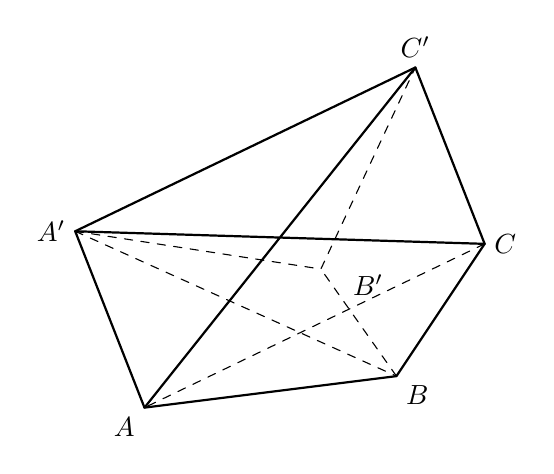
\begin{tikzpicture}[x=0.8cm,y=0.8cm,line cap=round,line join=round]
  \coordinate (A)  at (0,0);
  \coordinate (B)  at (4,0.5);
  \coordinate (C)  at (5.4,2.6);
  \coordinate (Ap) at (-1.1,2.8);
  \coordinate (Bp) at (2.8,2.2);
  \coordinate (Cp) at (4.3,5.4);
  % 底面三角形
  \draw[thick] (A)--(B)--(C);
  \draw[dashed] (C)--(A);
  % 上底面：A'C' 实线，其余两棱虚线
  \draw[thick] (Ap)--(Cp);
  \draw[dashed] (Ap)--(Bp)--(Cp);
  % 侧棱：AA'、CC' 实线，BB' 虚线
  \draw[thick] (A)--(Ap) (C)--(Cp);
  \draw[dashed] (B)--(Bp);
  % 两条对角实线 A'C、AC' 与虚线 A'B
  \draw[thick] (Ap)--(C) (A)--(Cp);
  \draw[dashed] (Ap)--(B);
  \node[below left] at (A) {$A$};
  \node[below right] at (B) {$B$};
  \node[right] at (C) {$C$};
  \node[left] at (Ap) {$A'$};
  \node at (3.55,1.95) {$B'$};
  \node[above] at (Cp) {$C'$};
\end{tikzpicture}
\end{center}
\nopagebreak[4]
\end{question}
\gksubpart{选做题：$A_2$组与$B_2$组二选一}

原卷说明：$A_2$组适合非试点校考生，$B_2$组适合试点校考生；考生从两组中选做一组。

\Needspace{0.4\textheight}
\begin{question}
\gkti{20}\textbf{（16分）} 本题共有 2 个小题。

$A_2$组（非试点校）：第 1 小题满分 8 分，第 2 小题满分 8 分。设虚数 $z_1,z_2$ 满足 $z_1^2=z_2$。

（1） 若 $z_1,z_2$ 又是一个实系数一元二次方程的两个根，求 $z_1,z_2$；

（2） 若 $z_1=1+mi$（$m>0$，$i$ 为虚数单位），$\omega=z_2-2$，$\omega$ 的辐角主值为 $\theta$，求 $\theta$ 的取值范围。

$B_2$组（试点校）：第 1 小题满分 6 分，第 2 小题满分 10 分。如图，抛物线 $C_1:y=-x^2$ 与抛物线 $C_2:y=x^2-2ax$（$a>0$）交于 $O,A$ 两点。

（1） 把 $C_1$ 与 $C_2$ 所围成的图形（阴影部分）绕 $x$ 轴旋转一周，求所得几何体的体积 $V$；

（2） 若过原点的直线 $l$ 与抛物线 $C_2$ 所围成的图形面积为 $\dfrac92a^3$，求直线 $l$ 的方程。
\nopagebreak[4]
\begin{center}% C1、C2 与阴影区域的示意重绘；图中取 a=1 仅为排布，非题设附加条件。
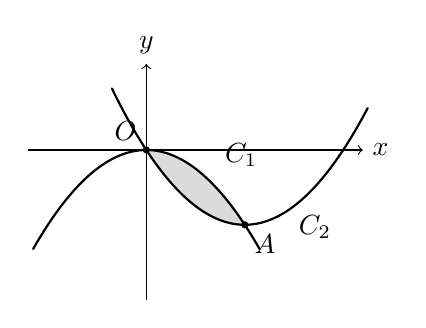
\begin{tikzpicture}[x=1.25cm,y=0.95cm,line cap=round,line join=round]
  \fill[gray!28] (0,0)
    -- plot[domain=0:1,samples=60] (\x,{ -\x*\x })
    -- plot[domain=1:0,samples=60] (\x,{ \x*\x-2*\x }) -- cycle;
  \draw[->] (-1.2,0)--(2.2,0) node[right] {$x$};
  \draw[->] (0,-2.0)--(0,1.15) node[above] {$y$};
  \draw[thick,domain=-1.15:1.15,samples=80] plot (\x,{ -\x*\x });
  \draw[thick,domain=-0.35:2.25,samples=80] plot (\x,{ \x*\x-2*\x });
  \fill (0,0) circle (1.3pt) node[above left] {$O$};
  \fill (1,-1) circle (1.3pt) node[below right] {$A$};
  \node[above right] at (0.7,-0.35) {$C_1$};
  \node[below right] at (1.45,-0.75) {$C_2$};
\end{tikzpicture}
\end{center}
\nopagebreak[4]
\Needspace{0.4\textheight}
\end{question}
\begin{question}
\gkti{21}\textbf{（18分）} 本题共有 3 个小题，第 1 小题满分 5 分，第 2 小题满分 6 分，第 3 小题满分 7 分。如图，抛物线方程为 $y^2=p(x+1)$（$p>0$），直线 $x+y=m$ 与 $x$ 轴的交点在抛物线的准线的右边。

（1） 求证：直线与抛物线总有两个交点；

（2） 设直线与抛物线的交点为 $Q,R$，$OQ\perp OR$，求 $p$ 关于 $m$ 的函数 $f(m)$ 的表达式；

（3） 在（2）的条件下，若 $m$ 变化使得原点 $O$ 到直线 $QR$ 的距离不大于 $\dfrac{\sqrt2}{2}$，求 $p$ 的取值范围。
\nopagebreak[4]
\begin{center}% 抛物线与弦示意；本图取 p=1、m=0.1，仅示关系，不按比例。
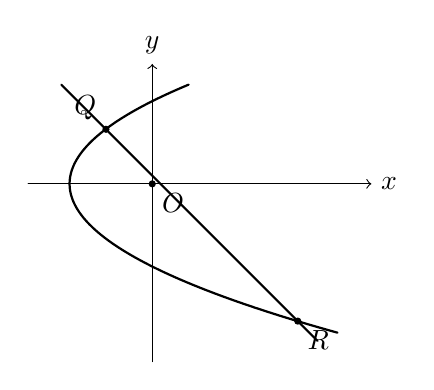
\begin{tikzpicture}[x=1.05cm,y=1.05cm,line cap=round,line join=round]
  \draw[->] (-1.5,0)--(2.65,0) node[right] {$x$};
  \draw[->] (0,-2.15)--(0,1.45) node[above] {$y$};
  \draw[thick,domain=-1.8:1.2,samples=90] plot ({\x*\x-1},{\x});
  \draw[thick,domain=-1.9:1.2,samples=80] plot ({0.1-\x},{\x});
  \fill (0,0) circle (1.3pt) node[below right] {$O$};
  \fill (-0.56,0.66) circle (1.3pt) node[above left] {$Q$};
  \fill (1.76,-1.66) circle (1.3pt) node[below right] {$R$};
\end{tikzpicture}
\end{center}
\nopagebreak[4]
\end{question}
\begin{question}
\gkti{22}\textbf{（18分）} 本题共有 3 个小题，每小题 6 分。设数列 $\{a_n\}$ 的首项 $a_1=1$，前 $n$ 项和 $S_n$ 满足关系式
\nopagebreak[4]
\[3tS_n-(2t+3)S_{n-1}=3t\qquad(t>0,\ n=2,3,4,\ldots).\]

（1） 求证：数列 $\{a_n\}$ 是等比数列；

\Needspace{5\baselineskip}
（2） 设数列 $\{a_n\}$ 的公比为 $f(t)$，作数列 $\{b_n\}$，使 $b_1=1$，$b_n=f\!\left(\dfrac1{b_{n-1}}\right)$（$n=2,3,4,\ldots$），求
\nopagebreak[4]
\[
\lim_{n\to\infty}\frac{\lg a_n}{b_n};
\]

（3） 求和：$b_1b_2-b_2b_3+b_3b_4-\cdots+(-1)^{n-1}b_nb_{n+1}$。

\end{question}